\documentclass[12pt]{article}

% packages
\usepackage{kantlipsum}
\usepackage[margin=1in]{geometry}
\usepackage[labelfont=it]{caption}
\usepackage[table]{xcolor}
\usepackage{subcaption,framed,colortbl,multirow}
\usepackage{amsmath,amsthm,amssymb,wasysym,mathrsfs,mathtools}
\usepackage{tikz,graphicx,pgf,pgfplots}
\usetikzlibrary{arrows, angles, quotes, decorations.pathreplacing, math, patterns, calc}
\pgfplotsset{compat=1.16}

\newtheorem{theorem}{Theorem}
\newtheorem{lemma}{Lemma}
\newtheorem{proposition}{Proposition}

% custom commands
\newcommand{\N}{\mathbb{N}}
\newcommand{\Z}{\mathbb{Z}}
\newcommand{\I}{\mathbb{I}}
\newcommand{\R}{\mathbb{R}}
\newcommand{\Q}{\mathbb{Q}}
\newcommand{\C}{\mathbb{C}}
\newcommand{\F}{\mathbb{F}}
\newcommand{\B}{\mathcal{B}}
\newcommand{\T}{\mathscr{T}}
\newcommand{\p}{^{\prime}}
\newcommand{\powerset}{\raisebox{.15\baselineskip}{\Large\ensuremath{\wp}}}
\DeclarePairedDelimiter{\ceil}{\lceil}{\rceil}
\DeclarePairedDelimiter\floor{\lfloor}{\rfloor}

\newcommand{\exercise}[2]{\section*{Exercise #1}\framebox{\begin{minipage}{\textwidth}#2\end{minipage}}\par\vspace{1em}}
\newcommand{\problem}[2]{\section*{Problem #1}\framebox{\begin{minipage}{\textwidth}#2\end{minipage}}\par\vspace{1em}}

\newenvironment{drawing}{\begin{center}\begin{tikzpicture}}{\end{tikzpicture}\end{center}}

\let\teq\trianglelefteq
\let\iso\cong % isomorphic (groups)

\title{depression}
\author{harrymcoleman }
\date{October 2019}

\begin{document}

\maketitle

\section*{sadness}
We'll define $S$ to be the set of all possible distances between any two points in the plane, ordered by $\leq$. We'll look at the greatest of these distances, call it $d$ and the two points which are $d$ units apart.

\begin{center}
    \begin{tikzpicture}
        \coordinate (A) at (0, 0);
        \coordinate (B) at (4, 0);
        \filldraw[black] (A) circle (2pt) node[anchor=east] {$A$};
        \filldraw[black] (B) circle (2pt) node[anchor=west] {$B$};
        
        \draw[dashed] (A) -- (B) node[anchor=south, midway] {$d$};
    \end{tikzpicture}
\end{center}

Since $d$ is the greatest distance between points in the plane, we know that no points will be anywhere farther than $d$ units from either $A$ or $B$.

\begin{center}
    \begin{tikzpicture}
        \coordinate (A) at (0, 0);
        \coordinate (B) at (4, 0);
        \filldraw[black] (A) circle (2pt) node[anchor=east] {$A$};
        \filldraw[black] (B) circle (2pt) node[anchor=west] {$B$};
        
        \draw[dashed] (A) -- (B) node[anchor=south, midway] {$d$};
        
        \draw[black] (A) circle (4cm);
        \draw[black] (B) circle (4cm);
        
    \end{tikzpicture}
\end{center}

This means that no points exist outside of the intersection of the circles shown. We'll simplify this to a rectangle, which actually includes some space where points cannot be.

\begin{center}
    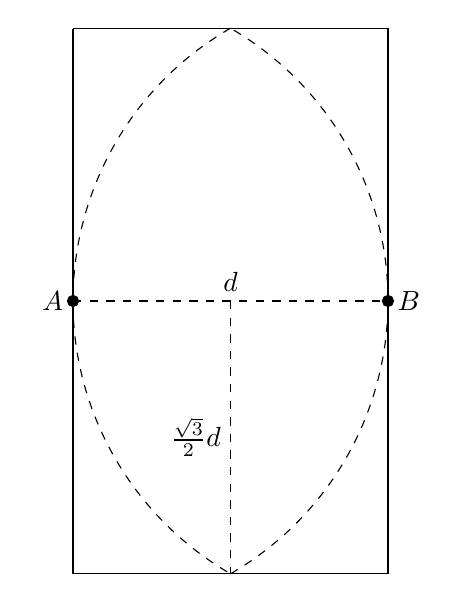
\begin{tikzpicture}
        \coordinate (A) at (0, 0);
        \coordinate (B) at (4, 0);
        \filldraw[black] (A) circle (2pt) node[anchor=east] {$A$};
        \filldraw[black] (B) circle (2pt) node[anchor=west] {$B$};
        
        \draw[dashed] (A) -- (B) node[anchor=south, midway] {$d$};
        
        \draw[dashed] ([shift=(-60:4cm)]0,0) arc (-60:60:4cm);
        \draw[dashed] ([shift=(120:4cm)]4,0) arc (120:240:4cm);
        
        \draw (0,3.46) -- (4,3.46) -- (4,-3.46) -- (0,-3.46) -- (0,3.46);
        
        \draw[dashed] (2,0) -- (2,-3.46) node[anchor=east, midway]{$\frac{\sqrt{3}}{2}d$};
        
    \end{tikzpicture}
\end{center}

This rectangle, as can be seen, has a width of $d$ units, and a height of $\sqrt{3}d$ units. Since $d$ is our maximum distance, the other points must also lie within a vertical range of $d$ units. We'll call $C$ the point which is farthest from segment $AB$ and orient the plane so it is on top.

\begin{center}
    \begin{tikzpicture}
        \coordinate (A) at (0, 0);
        \coordinate (B) at (4, 0);
        \filldraw[black] (A) circle (2pt) node[anchor=east] {$A$};
        \filldraw[black] (B) circle (2pt) node[anchor=west] {$B$};
        \draw (0,3.46) -- (4,3.46) -- (4,-3.46) -- (0,-3.46) -- (0,3.46);
        \draw (2,3.46) node[anchor=south] {d};
        \draw[decorate, decoration={brace, amplitude=10}] (4.5,3.46) -- (4.5,-3.46) node[anchor=west, midway, xshift=10pt]{$\sqrt{3}d$};
        
        \coordinate (C) at (1.5,2);
        \filldraw[black] (C) circle (2pt) node[anchor=south] {$C$};
        
        \draw[dashed] (0,2) -- (4,2);
        \draw[dashed] (0,-2) -- (4,-2);
        
        \draw[dashed] (C) -- (1.5,-2) node[anchor=west, midway]{$d$};
    \end{tikzpicture}
\end{center}

Since $C$ is our topmost point, there can be no points above it. And since $d$ is our maximum distance, there can be no points farther than $d$ units below $C$. This shrinks the overall area where points can be to a square with sidelength $d$ units.

\begin{center}
    \begin{tikzpicture}
        \coordinate (A) at (0, 0);
        \coordinate (B) at (4, 0);
        \filldraw[black] (A) circle (2pt) node[anchor=east] {$A$};
        \filldraw[black] (B) circle (2pt) node[anchor=west] {$B$};
        \draw (0,2) -- (4,2) -- (4,-2) -- (0,-2) -- (0,2);
        \draw (2,2) node[anchor=south] {$d$};
        \draw[decorate, decoration={brace, amplitude=10}] (4.5,2) -- (4.5,-2) node[anchor=west, midway, xshift=10pt]{$d$};
    \end{tikzpicture}
\end{center}

If $d \leq \sqrt{2}$, it is trivial to show that all the points are inside a triangle of area less than or equal to 4.

\begin{center}
    \begin{tikzpicture}
        \coordinate (A) at (0, 0);
        \coordinate (B) at (4, 0);
        \filldraw[black] (A) circle (2pt) node[anchor=east] {$A$};
        \filldraw[black] (B) circle (2pt) node[anchor=west] {$B$};
        \draw (0,2) -- (4,2) -- (4,-2) -- (0,-2) -- (0,2);
        \draw (2,2) node[anchor=south] {$d$};
        \draw[decorate, decoration={brace, amplitude=10}] (4.5,2) -- (4.5,-2) node[anchor=west, midway, xshift=10pt]{$d$};
        
        \draw[dashed] (0,-2) -- (-4,-2) -- (4, 6) -- (4,2);
    \end{tikzpicture}
\end{center}

With $d \leq \sqrt{2}$, the square would have an area less than or equal to 2, and each smaller triangle an area less than or equal to 1, giving the overall triangle an area less than or equal to 4. So we'll consider $d>\sqrt{2}$ for the rest of the process.

Now considering the main property of our points, any 3 points forms a triangle of area less than or equal to 1. Considering this, we want to know what the maximum height of our bounding box is. 

\begin{center}
    \begin{tikzpicture}
        \coordinate (A) at (0, 0);
        \coordinate (B) at (4, 0);
        \filldraw[black] (A) circle (2pt) node[anchor=east] {$A$};
        \filldraw[black] (B) circle (2pt) node[anchor=west] {$B$};
        \draw (0,2) -- (4,2) -- (4,-2) -- (0,-2) -- (0,2);
        
        \coordinate (C) at (2,2);
        \filldraw[black] (C) circle (2pt) node[anchor=south] {$C$};
        
        \draw[dashed] (A) -- (C) -- (B);
        \draw[dashed] (A) -- (B) node[anchor=north, midway] {$d$};
        \draw[dashed] (C) -- (2,0) node[anchor=west, midway] {$h$};
        
        \draw[decorate, decoration={brace, amplitude=10}] (4.5,2) -- (4.5,-2) node[anchor=west, midway, xshift=10pt]{$2h$};
    \end{tikzpicture}
\end{center}

The area of triangle $ABC$ is 

\[\frac{1}{2}dh \leq 1\]
so
\[h \leq \frac{2}{d}\]

So the area of our rectangle is 
\[2hd \leq 2\frac{2}{d}d\]
\[2hd \leq 4\]

To squeeze the possible area of points even more, we're going to look at the corners of our rectangle. The dotted lines connect each of the midpoints of the sides of our rectangle to each other.

\begin{center}
    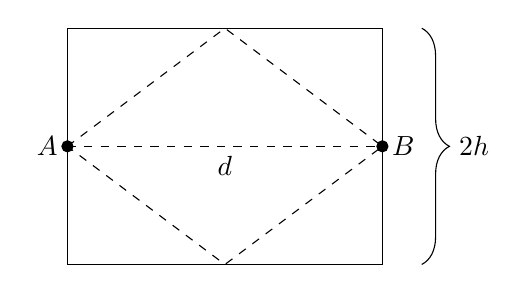
\begin{tikzpicture}
        \coordinate (A) at (0, 0);
        \coordinate (B) at (4, 0);
        \filldraw[black] (A) circle (2pt) node[anchor=east] {$A$};
        \filldraw[black] (B) circle (2pt) node[anchor=west] {$B$};
        \draw (0,1.5) -- (4,1.5) -- (4,-1.5) -- (0,-1.5) -- (0,1.5);
        
        
        \draw[dashed] (A) -- (2,1.5) -- (B) -- (2,-1.5) -- (A);
        \draw[dashed] (A) -- (B) node[anchor=north, midway] {$d$};
        
        \draw[decorate, decoration={brace, amplitude=10}] (4.5,1.5) -- (4.5,-1.5) node[anchor=west, midway, xshift=10pt]{$2h$};
    \end{tikzpicture}
\end{center}

\begin{center}
    \begin{tikzpicture}
        \coordinate (A) at (0, 0);
        \coordinate (B) at (4, 0);
        \coordinate (C) at (3, 3);
        \filldraw[black] (A) circle (2pt) node[anchor=east] {$A$};
        \filldraw[black] (B) circle (2pt) node[anchor=west] {$B$};
        \filldraw[black] (C) circle (2pt) node[anchor=south] {$C$};
        
        \draw[black] (A) -- (B) -- (C) -- (A);
        
        \coordinate (c1) at (-2,3);
        \coordinate (c2) at (8,3);
        
        \coordinate (b1) at (8,4);
        \coordinate (b2) at (0,-4);
        
        \coordinate (a1) at (1.33, -4);
        \coordinate (a2) at (-1.33, 4);
        
        \draw[dashed] (c1) -- (c2);
        \draw[dashed] (b1) -- (b2);
        \draw[dashed] (a1) -- (a2);
        
        \coordinate (ap) at (7,3);
        \pic [draw, ->, "$\alpha$", angle eccentricity=1.5] {angle = B--A--C};
        \pic [draw, ->, "$\alpha$", angle eccentricity=1.5] {angle = c2--ap--b1};
        \pic [draw, ->, "$\alpha$", angle eccentricity=1.5] {angle = C--ap--B};
        
        \coordinate (bp) at (-1,3);
        \pic [draw, ->, "$\beta$", angle eccentricity=1.5] {angle = C--B--A};
        \pic [draw, ->, "$\beta$", angle eccentricity=1.5] {angle = a2--bp--c1};
        \pic [draw, ->, "$\beta$", angle eccentricity=1.5] {angle = A--bp--C};
        
        \coordinate (cp) at (1,-3);
        \pic [draw, ->, "$\gamma$", angle eccentricity=1.5] {angle = A--C--B};
        \pic [draw, ->, "$\gamma$", angle eccentricity=1.5] {angle = b2--cp--a1};
        \pic [draw, ->, "$\gamma$", angle eccentricity=1.5] {angle = B--cp--A};
        
        \filldraw[black] (ap) circle (2pt) node[anchor=north] {$A^\prime$};
        \filldraw[black] (bp) circle (2pt) node[anchor=north east] {$B^\prime$};
        \filldraw[black] (cp) circle (2pt) node[anchor=east] {$C^\prime$};
        
        
        
    \end{tikzpicture}
\end{center}


\section{squar}

\begin{figure}[ht]
    \centering
    \begin{subfigure}[b]{.47\textwidth}
        \centering
        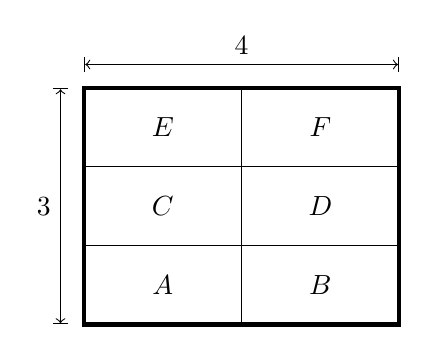
\begin{tikzpicture}
            \draw[|<->|] (-0.3,0) -- (-0.3,3) node[midway, anchor=east]{3};
            \draw[|<->|] (0,3.3) -- (4,3.3) node[midway, anchor=south]{4};
            \draw[ultra thick] (0,0) rectangle (4,3);
            
            \draw[] (0,1)--(4,1) (0,2)--(4,2) (2,0)--(2,3);
            %\draw[dashed] (1,0)--(1,3) (3,0)--(3,3);
            
            \foreach \x/\y/\n in {1/0.5/A, 3/0.5/B, 1/1.5/C, 3/1.5/D, 1/2.5/E, 3/2.5/F} {
                \draw[] (\x,\y) node[]{$\n$};
            }
            
        \end{tikzpicture}
        \caption{six $1\times2$ rectangles}
        \label{fig:parts-12}
    \end{subfigure}
    \begin{subfigure}[b]{.47\textwidth}
        \centering
        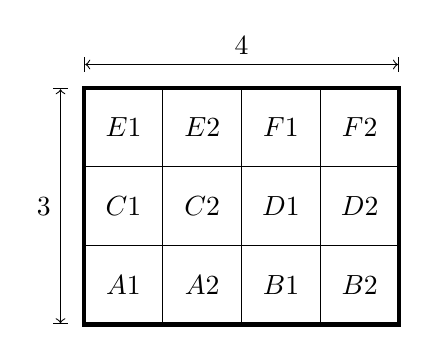
\begin{tikzpicture}
            \draw[|<->|] (-0.3,0) -- (-0.3,3) node[midway, anchor=east]{3};
            \draw[|<->|] (0,3.3) -- (4,3.3) node[midway, anchor=south]{4};
            \draw[ultra thick] (0,0) rectangle (4,3);
            
            \draw[] (0,1)--(4,1) (0,2)--(4,2) (2,0)--(2,3) (1,0)--(1,3) (3,0)--(3,3);
            
            \foreach \x/\y/\n in {0/0/A1, 1/0/A2, 2/0/B1, 3/0/B2, 0/1/C1, 1/1/C2, 2/1/D1, 3/1/D2, 0/2/E1, 1/2/E2, 2/2/F1, 3/2/F2} {
                \draw[] (\x+0.5,\y+0.5) node[]{$\n$};
            }
            
        \end{tikzpicture}
        \caption{twelve $1\times1$ squares}
        \label{fig:parts-squares}
    \end{subfigure}
    \caption{A $3\times4$ rectangle partitioned in two ways.}
    \label{fig:parts-34}
\end{figure}



\section{max}
We will denote each of the elementary row operations on a matrix $A$ in the following ways:
\begin{itemize}
    \item $P_{ij}(A)$ Permute rows $i$ and $j$.
    \item $M_{i(\alpha)}(A)$ Multiply row $i$ by $\alpha$.
    \item $R_{ij(\alpha)}(A)$ Replace row $i$ by the sum of row $i$ and the product of $\alpha$ and row $j$.
\end{itemize}
\vspace{1em}

Let $A\in\F^{m\times n}$, where
\[A =
    \begin{bmatrix}
        a_{11} & a_{12} & a_{13} & \cdots & a_{1m} \\
        a_{21} & a_{22} & a_{23} & \cdots & a_{2m} \\
        a_{31} & a_{32} & a_{33} & \cdots & a_{3m} \\
        \vdots & \vdots & \vdots & \ddots & \vdots \\
        a_{n1} & a_{n2} & a_{n3} & \cdots & a_{nm} \\
    \end{bmatrix}
.\]

For this arbitrary matrix, we will give a series of row operations which will produce a matrix in row echelon form. By definition, these two matrices will be row-equivalent. 

To begin, we find the first column $j$ with nonzero elements, and the first nonzero element $a_{ij}$ in that column. This means that all elements above $a_{ij}$ in the $j$th column are zero, and all elements in columns to the left of the $j$th column are zero. We will call $a_{ij}$ the \emph{guide} element for the next few steps, and refer to it by $g$, since it will not necessarily stay in the $i$th row and $j$th column during this process. The process for operating on $A$ are given in the following steps:

\vspace{1em}
\noindent
\framebox{\begin{minipage}{\textwidth}
    \begin{enumerate}
        \item If $i\ne1$, then take $A' = P_{i1}(A)$ so that the guide becomes the first nonzero element in the first row. Otherwise, take $A'=A$.
        
        \item For each row $k>1$, apply $R_{k1(d)}$ to $A'$ where
        \[d = \frac{-A'_{kj}}{g}.\]
        Call the resultant matrix of these operations $A^1$.
    \end{enumerate}
\end{minipage}}\vspace{1em}

The second step ensures that for each row $k>1$,
\[A^1_{kj} = A'_{kj} + \left(\frac{-A'_{kj}}{g}\right)g = A'_{kj} - A'_{kj} = 0.\]

So $A^1$ is a matrix in which every element below the guide is zero\textemdash that is,
\[A^1 =
    \begin{bmatrix}
        0      & \cdots & 0      & a^1_{1j} & a^1_{1(j+1)}  & \cdots & a^1_{1m}  \\
        \vdots & \ddots &        & 0      & \vdots      & \ddots & \vdots  \\
        \vdots &        & \ddots & \vdots & \vdots      & \ddots & \vdots  \\
        0      & \cdots & \cdots & 0      & a^1_{n(j+1)} & \cdots & a^1_{nm} \\
    \end{bmatrix}
.\]

It can be seen that $A^1$ is starting to look like a matrix in echelon form. We continue by finding a new guide element $g^1$, this time only considering rows below the first, and columns to the right of $j$. 

In general, to find the guide $g^s$ at step $s$, we look for the first column from the left which has nonzero elements in rows greater than $s-1$. Then in that column $q$, we take the nonzero element $a^s_{pq}$ such that for all $k$ with $s<k<p$, we have $a^s_{kq}=0$. This $a^s_{pq}$ will be the new guide $g^s$.

We now perform the below algorithm with matrix $A^1$ and guide $g^1$.

\vspace{1em}
\noindent
\framebox{\begin{minipage}{\textwidth}
    For a given matrix $A^s$ and guide element $g^s=A^s_{ij}$, do the following:
    
    \begin{enumerate}
        \item If $i\ne s$, then take $A^{s\prime} = P_{is}(A^s)$ so that the guide becomes the first nonzero element in row $s$. Otherwise, take $A^{s\prime}=A^s$.
        
        \item For each row $k>1$, apply $R_{k1(d)}$ to $A^{s\prime}$ where
        \[d = \frac{-A^{s\prime}_{kj}}{g^s}.\]
        Call the resultant matrix of these operations $A^{s+1}$.
        
        \item If $A^{s+1}$ is not in echelon form, repeat steps 1-3 for matrix $A^{s+1}$ and a new guide $g^{s+1}$.
    \end{enumerate}
\end{minipage}}\vspace{1em}

From this process, we find
\[A^2 =
    \begin{bmatrix}
        g^1    & *      & \cdots & \cdots & * \\
        0      & g^2    & *      & \cdots & *   \\
        \vdots & 0      & \vdots & \ddots & \vdots   \\
        \vdots & \vdots & \vdots & \ddots & \vdots   \\
        0      & 0      & *      & \cdots & * \\
    \end{bmatrix}
.\]
(Note that in the above depiction of $A^2$, numerous zero columns might exist before the first shown column, and some columns with zeros below the first row might exist between the first two shown columns. Unspecified elements in $\F$ are denoted by $*$.)

As can be seen, at each step, the algorithm produces a matrix with an additional row which satisfies the conditions for echelon form. Eventually, the process will run out of rows or columns, and will halt on some matrix $A^t$ that is in echelon form. Because this matrix is obtained by a series of row operations on $A$, it is row-equivalent to $A$.

Therefore, any matrix is row-equivalent to some matrix in echelon form.


\section{bop}

Supposing that $V$ and $W$ are finite-dimensional, we want to show that $L(V,W)$ is also finite-dimensional. We will do so by providing a finite basis. First let
\[\beta_V = \{v_1, \dots, v_n\}\]
be a finite basis for $V$ and define the linear functional $P\in L(V,\F)$ in the following way: for all $x\in V$, where
\[x = \alpha_1 v_1 + \cdots + \alpha_n v_n\]
is the unique linear combination of vectors in $\beta_V$, we assign $P(x)=\alpha_1$. In other words, for all $x\in V$, $P(x)=\alpha_1$ where $\alpha_1v_1$ is the projection of $x$ on span$(v_1)$ along span$\{v_2,\dots,v_n\}$. $P$ inherits its linearity from that of projection. For simplicity, we define $\alpha_x := P(x)$ for all $x\in V$. Now let
\[\beta_W = \{w_1, \dots, w_m\}\]
be a finite basis for $W$. And let
\[\B = \{B_1, \dots, B_m\} \subseteq L(V,W)\]
where $B_i(x) = \alpha_x w_i$ for all $x\in V$. Each $B_i$ inherits its linearity from $P$ since for all $x,y\in V$,
\begin{align*}
    B_i(x+y)    &= \alpha_{x+y}w_i, \\
                &= (\alpha_x + \alpha_y)w_i, \\
                &= \alpha_x w_i + \alpha_y w_i, \\
                &= B_i(x) + B_i(y).
\end{align*}
And for all $\gamma\in\F$,
\begin{align*}
    B_i(\gamma x)   &= \alpha_{\gamma x}w_i, \\
                    &= \gamma\alpha_x w_i, \\
                    &= \gamma B_i(x).
\end{align*}

We now show that $\B$ is a basis for $L(V,W)$. Suppose for some $\gamma_1, \dots, \gamma_m\in\F$,
\[\gamma_1 B_1 + \cdots + \gamma_m B_m = \textbf{0}.\]
By our definitions, this means that for all $x\in V$,
\begin{align*}
    [\gamma_1 B_1 + \cdots + \gamma_m B_m](x)               &= \textbf{0}(x), \\
    \gamma_1 \alpha_x w_1 + \cdots + \gamma_m \alpha_x w_m  &= 0_W, \\
    \gamma_1 w_1 + \cdots + \gamma_m w_m                    &= 0_W.
\end{align*}
Since $\beta_W$ is linearly independent, all $\gamma_i=0_\F$, therefore $\B$ is linearly independent. Now let $F\in L(V,W)$ and $x\in V$. Since $F(x)\in W$, for some $\delta_1,\dots,\delta_m\in\F$, we have
\[F(x) = \delta_1 w_1 + \cdots + \delta_m w_m.\]
For each $i$, we define $\gamma_i = \frac{\delta_i}{\alpha_x}$, which gives us
\[F(x) = \gamma_1 \alpha_x w_1 + \cdots + \gamma_m \alpha_x w_m,\]
\[F(x) = \gamma_1 B_1 + \cdots + \gamma_m B_m.\]
So $\B$ generates $L(V,W)$. Since $\B$ is a linearly independent generating set, it is a basis for $L(V,W)$. This means that $L(V,W)$ is a finite-dimensional vector space with dimension equal to that of $W$.


\section{cattttttt}
\begin{drawing}
    \foreach \x in {0,4,8} {
        \draw (\x,0) node{$C$};
    }
    \draw (6,2) node{$C$};
    
    \draw[->] (0.5,0)--(3.5,0)node[midway,anchor = south]{$T$};
    \draw[->] (4.5,0)--(7.5,0)node[midway,anchor = south]{$T$};
    
    \draw[->] (4.25,0.25)--(5.75,1.75)node[midway,anchor=south east]{$T$};
    \draw[->] (6.25,1.75)--(7.75,0.25)node[midway,anchor=south west]{$T$};
    
    \draw (6,1)node{$\Downarrow\mu$};
    
    \draw[->] (0.25,-0.25)to[out=-30,in=210](7.75,-0.25);
    \draw (4,-1.75) node{$T$};
    \draw (4,-0.75)node{$\Downarrow\mu$};
\end{drawing}

\begin{drawing}
    \foreach \x in {0,4,8} {
        \draw (\x,0) node{$C$};
    }
    \draw (2,2) node{$C$};
    
    \draw[->] (0.5,0)--(3.5,0)node[midway,anchor = south]{$T$};
    \draw[->] (4.5,0)--(7.5,0)node[midway,anchor = south]{$T$};
    
    \draw[->] (0.25,0.25)--(1.75,1.75)node[midway,anchor=south east]{$T$};
    \draw[->] (2.25,1.75)--(3.75,0.25)node[midway,anchor=south west]{$T$};
    
    \draw (2,1)node{$\Downarrow\mu$};
    
    \draw[->] (0.25,-0.25)to[out=-30,in=210](7.75,-0.25);
    \draw (4,-1.75) node{$T$};
    \draw (4,-0.75)node{$\Downarrow\mu$};
\end{drawing}


\section{toop}

We define a family of subsets $\T$ of $\R$ as follows
    \[\T = \left\{\bigcup_{\alpha\in I}U_\alpha : \{U_\alpha : \alpha\in I\} \subseteq \B\right\}.\]
    By its definition, if $\T$ is a topology on $\R$, then $\B$ is indeed a topological base for $\T$. Not that $\emptyset \in \T$ as the empty set is the union of an empty collection of sets of $\B$. And since we can construct the following union:
    \[\bigcup_{n=1}^\infty[-n,n) = \R,\]
    then $\R\in\T$. Suppose $\{\mathcal{U}_\beta: \beta\in J\}$ is a collection of open subsets in $\T$, that is,
    \[\mathcal{U}_\beta = \bigcup_{\alpha\in I_\beta}U_\alpha,\]
    where $\{u_\alpha : \alpha\in I_\beta\}$ is a subset of $\B$. Then if we define
    \[I = \bigcup_{\beta \in J}I_\beta,\]
    then
    \[\bigcup_{\beta \in J}\mathcal{U}_\beta = \bigcup_{\beta \in J}\bigcup_{\alpha\in I_\beta}U_\alpha = \bigcup_{\alpha\in I}U_\alpha.\]
    And since $\{U_\alpha : \alpha \in I\}$ is a subset of $\B$, then we have
    \[\bigcup_{\beta \in J}\mathcal{U}_\beta \in \T.\]


\section{balogna}

\begin{proposition}
    $(C\times D)\teq(A\times B)$.
\end{proposition}

\begin{proof}
    Suppose $(a,b)\in (A\times B)$. Since $C\teq A$ and $D\teq B$, then by the definition of cosets and multiplication in the direct product group, we have
    \begin{align*}
        (a,b)(C\times D) 
            &= \{(a,b)(c,d) : c\in C, d\in D\} \\
            &= \{(ac,bd) : c\in C, d\in D\} \\
            &= (aC, bD) \\
            &= (Ca, Db) \\
            &= \{(ca,db) : c\in C, d\in D\} \\
            &= \{(c,d)(a,b) : c\in C, d\in D\} \\
            &= (C\times D)(a,b).
    \end{align*}
    Thus, $(C\times D)\teq(A\times B)$.

\end{proof}

\begin{proposition}
    $(A\times B)/(C\times D) \iso (A/C)\times(B/D)$.
\end{proposition}

We denote by $1_A$ the function in $A$ which maps all elements of $X$ to $1_G$, i.e., $1_A(x)=1_G$ for all $x\in X$. This is, indeed, the identity of $A$, since for any $f\in A$ and $x\in X$, we have
    \[(1_Af)(x) = 1_A(x)f(x) = 1_Gf(x) = f(x).\]
    For any $f\in A$, we denote by $f^{-1_A}$ function of $A$ which maps $f^{-1_A}(x) = (f(x))^{-1}$ for all $x\in X$. We can see that $f^{-1_A}$ is the inverse of $f$, since for any $x\in X$, we have
    \[(f^{-1_A}f)(x) = f^{-1_A}(x)f(x) = (f(x))^{-1}f(x) = 1_G = 1_A(x).\]
    
    Now let $f\in A$, and we consider the set $fA_0f^{-1_A}$. For any $g\in A_0$, we have
    \begin{align*}
        (fgf^{-1_A})(x_0) 
            &= f(x_0)(gf^{-1_A})(x_0) \\
            &= f(x_0)g(x_0)f^{-1_A}(x_0) \\
            &= f(x_0)1_G(f(x_0))^{-1} \\
            &= f(x_0)(f(x_0))^{-1} \\
            &= 1_G.
    \end{align*}
    This implies that $fgf^{-1_A} \in A_0$, so $fA_0f^{-1_A}\subseteq A_0$ and $A_0\teq A$. 
    
\section*{splingle}

\begin{align*}
    f[\sigma(x_0),\dots,\sigma(x_n)]
    &= \sum_{j=0}^n \frac{f(\sigma(x_j))}{\displaystyle\prod_{\substack{k=0 \\ k\ne j}}^n (\sigma(x_j)-\sigma(x_k))} \\
    &= \frac{f(\sigma(x_a))}{\displaystyle\prod_{\substack{k=0 \\ k\ne a}}^n (\sigma(x_a)-\sigma(x_k))}
        + \frac{f(\sigma(x_b))}{\displaystyle\prod_{\substack{k=0 \\ k\ne b}}^n (\sigma(x_b)-\sigma(x_k))}
        +\sum_{\substack{j=0 \\ j\ne a \\ j\ne b}}^n \frac{f(\sigma(x_j))}{\displaystyle\prod_{\substack{k=0 \\ k\ne j}}^n (\sigma(x_j)-\sigma(x_k))} \\
    &= \frac{f(x_b)}{\displaystyle\prod_{\substack{k=0 \\ k\ne a}}^n (x_b-\sigma(x_k))}
        + \frac{f(x_a)}{\displaystyle\prod_{\substack{k=0 \\ k\ne b}}^n (x_a-\sigma(x_k))}
        +\sum_{\substack{j=0 \\ j\ne a \\ j\ne b}}^n \frac{f(x_j)}{\displaystyle\prod_{\substack{k=0 \\ k\ne j}}^n (x_j-\sigma(x_k))} \\
    &= \frac{f(x_b)}{(x_b-\sigma(x_b))\displaystyle\prod_{\substack{k=0 \\ k\ne a \\ k\ne b}}^n (x_b-\sigma(x_k))}
        + \frac{f(x_a)}{(x_a - \sigma(x_a))\displaystyle\prod_{\substack{k=0 \\ k\ne b \\ k\ne a}}^n (x_a-\sigma(x_k))}
        +\sum_{\substack{j=0 \\ j\ne a \\ j\ne b}}^n \frac{f(x_j)}{(x_j-\sigma(x_a))(x_j-\sigma(x_b))\displaystyle\prod_{\substack{k=0 \\ k\ne j \\ k\ne a \\ k\ne b}}^n (x_j-\sigma(x_k))} \\
    &= \frac{f(x_b)}{(x_b-x_a)\displaystyle\prod_{\substack{k=0 \\ k\ne a \\ k\ne b}}^n (x_b-x_k)}
        + \frac{f(x_a)}{(x_a - x_b)\displaystyle\prod_{\substack{k=0 \\ k\ne b \\ k\ne a}}^n (x_a-x_k)}
        +\sum_{\substack{j=0 \\ j\ne a \\ j\ne b}}^n \frac{f(x_j)}{(x_j-x_b)(x_j-x_a)\displaystyle\prod_{\substack{k=0 \\ k\ne j \\ k\ne a \\ k\ne b}}^n (x_j-x_k)} \\
    &= \frac{f(x_b)}{\displaystyle\prod_{\substack{k=0 \\ k\ne b}}^n (x_b-x_k)}
        + \frac{f(x_a)}{\displaystyle\prod_{\substack{k=0 \\ k\ne a}}^n (x_a-x_k)}
        +\sum_{\substack{j=0 \\ j\ne a \\ j\ne b}}^n \frac{f(x_j)}{\displaystyle\prod_{\substack{k=0 \\ k\ne j}}^n (x_j-x_k)} \\
    &= \sum_{j=0}^n \frac{f(x_j)}{\displaystyle\prod_{\substack{k=0 \\ k\ne j}}^n (x_j-x_k)} \\
    &= f[x_0,\dots,x_n].
\end{align*}

\section{probbababababa}

\begin{proposition}
    If $X \overset{d}{=} \operatorname{Bin}(n, p)$ for $n\in\N$ and $p\in(0, 1)$, then $X(\Omega) = \{0, \dots, n\}$.
\end{proposition}

\begin{proof}
    We will use the fact that $k \in X(\Omega)$ if and only if $\P(X = k) > 0$. Suppose $k \in \{0, \dots, n\}$, then
    \[\P(X = k) = \binom{n}{k}p^k(1-p)^{n-k}.\]
    Now since $p \in (0, 1)$, then $p^k > 0$ and $(1-p)^{n-k} > 0$, and since $k \in \{0, \dots, n\}$, then $\binom{n}{k} > 0$. Thus, we have $\P(X = k) > 0$, which implies $k \in X(\Omega)$. This proves that $\{0, \dots, n\} \subseteq X(\Omega)$, and the opposite inclusion remains.
    
    To prove that $X(\Omega) \subseteq \{0,\dots, n\}$, we will prove the equivalent statement $\R \setminus \{0, \dots, n\} \subseteq \R \setminus X(\Omega)$. Suppose $a \in \R \setminus \{0, \dots, n\}$, and we consider the probability
    \[\P(X \in \{0, \dots, n, a\}) = \P(X^{-1}(0) \cup \cdots \cup X^{-1}(n) \cup X^{-1}(a)).\]
    Clearly the preimages of $X$ are disjoint; if this were not true, then there would be some $\omega \in \Omega$ with multiple images under the function $X$, which would be a contradiction. Thus,
    \begin{align*}
        \P(X \in \{0, \dots, n, a\})
            &= \P(X^{-1}(0)) + \cdots + \P(X^{-1}(n)) + \P(X^{-1}(a)) \\[1em]
            &= \P(X = 0) + \cdots + \P(X = n) + \P(X = a) \\[1em]
            &= \P(X = a) + \sum_{k=0}^n \P(X = k) \\[1em]
            &= \P(X = a) + \sum_{k=0}^n \binom{n}{k}p^k(1-p)^{n-k} \\[1em]
            &= \P(X = a) + (p + 1 - p)^n \\[1em]
            &= \P(X = a) + 1.
    \end{align*}
    Because the probability function is a map $\P:\Omega \to [0, 1]$, then 
    \[\P(X = a) \in [0, 1] \isp{and} \P(X \in \{0, \dots, n, a\}) \in [0, 1].\]
    The above equality now implies that $P(X = a) \in [-1, 0]$, so we must have $P(X = a) = 0$. Therefore, $a \notin X(\Omega)$, so $a \in \R \setminus X(\Omega)$ and the proof is complete.
    
\end{proof}

\section{apalachian}

Let $a_n$ denote the non-alternating part of the $n$th term of the series (2), i.e.,
    \[
        a_n = \frac{\sqrt{n+1} - \sqrt{n}}{n}
    \]
    We first show that the series converges. For any $n \in \N$, we have
    \begin{align*}
        n &\leq n + 1, \\
        \sqrt{n} &\leq \sqrt{n + 1}, \\
        0 &\leq \sqrt{n + 1} - \sqrt{n}, \\
        0 &\leq \frac{\sqrt{n + 1} - \sqrt{n}}{n}, \\
        0 &\leq a_n.
    \end{align*}
    Therefore, the series (2), which can be written as
    \[
        \sum_{n=1}^\infty (-1)^n a_n,
    \]
    converges if $a_n \to 0$. We first note that for all $n \in \N$,
    \[
        \sqrt{n + 1}-\sqrt{n}  = \frac{n + 1 - n}{\sqrt{n + 1} + \sqrt{n}} = \frac{1}{\sqrt{n + 1} + \sqrt{n}}\leq 1.
    \]
    Then, we find that
    \[
        0 \leq a_n = \frac{\sqrt{n+1} - \sqrt{n}}{n} \leq \frac1n.
    \]
    And since $\frac1n \to 0$, then by the squeeze theorem, $a_n \to 0$. Thus, the alternating series (2) converges. On the other hand, we now consider the absolute value of the terms in the series. For any $n \in \N$, we have
    \[
        \left| (-1)^n a_n \right| = a_n = \frac{\sqrt{n+1} - \sqrt{n}}{n} \geq \frac{\sqrt{n+1}}{n} \geq \frac1n.
    \]

    By definition, $\alpha$ and $\beta$ are the greatest subsequential limits of $\seq{a_n}$ and $\seq{b_n}$, respectively. Likewise,
    \[
        \gamma = \limsup _{n\to \infty} (a_n+b_n),
    \]
    where $\gamma \in \R \cup \{\pm \infty\}$ is the greatest subsequential limit of $\seq{a_n + b_n}$. Let $\seq[k]{a_{n_k} + b_{n_k}}$ be a subsequence such that
    \[
        a_{n_k} + b_{n_k} \to \gamma.
    \]
    We consider the corresponding pair of subsequences given by $\seq[k]{a_{n_k}}$ and $\seq[k]{b_{n_k}}$. We now take a subsequence $\seq[i]{a_{n_i}} \subseteq \seq[k]{a_{n_k}}$ such that
    \[
        a_{n_i} \to \alpha' \in \R \cup \{\pm \infty\}.
    \]
    And a further subsequence $\seq[j]{b_{n_j}} \subseteq \seq[i]{b_{n_i}}$ such that
    \[
        b_{n_j} \to \beta' \in \R \cup \{\pm \infty\}.
    \]
    Thus, we now have
    \[
        a_{n_j} \to \alpha', \quad b_{n_j} \to \beta', \quad a_{n_j} + b_{n_j} \to \gamma.
    \]
    This implies that $\gamma = \alpha' + \beta'$. And since $\alpha'$ and $\beta'$ are subsequential limits of $\seq{a_n}$ and $\seq{b_n}$, respectively, we obtain the desired results $\gamma \leq \alpha + \beta$.
    
    We will prove, by induction that $\sqrt{a} < x_{n + 1} < x_n$ for all $n \in \N$. For the base case, we are given $\sqrt{a} < x_1$. (It will become clear that this base case is sufficient, as the fact that $\sqrt{a} < x_2 < x_1$ is an instance of the inductive step.) Suppose we have $\sqrt{a} < x_n$, then
    \[
        x_{n + 1} = \frac{1}{2} \left( x_n + \frac{a}{x_n} \right) < \frac{1}{2} \left( x_n + \frac{a}{\sqrt{a}} \right) = \frac{x_n + \sqrt{a}}{2} < \frac{x_n + x_n}{2} = x_n.
    \]
    Thus, $x_{n + 1} < x_n$. We now use this fact and the fact that $\sqrt{a} < x_n$ to derive
    \[
        x_{n + 1} = \frac{1}{2} \left( x_n + \frac{a}{x_n} \right) > \frac{1}{2} \left( x_{n + 1} + \frac{a}{\sqrt{a}} \right) = \frac{x_{n + 1} + \sqrt{a}}{2}.
    \]
    And solving for $x_{n + 1}$, we obtain $\sqrt{a} < x_{n + 1}$, completing the induction.


\section{dense}

\[
    F_X(s) = \begin{cases}
        0 & -\infty < s < 1 \\
        1/16 & \phantom{-x}1 \leq s < 2 \\
        4/16 & \phantom{-x}2 \leq s < 3 \\
        9/16 & \phantom{-x}3 \leq s < 4 \\
        1 & \phantom{-x}4 \leq s < \infty.
    \end{cases}
\]

\begin{align*}
    F_X : (-\infty, 1) &\mapsto 0 \\
    [1, 2) &\mapsto 1/16 \\
    [2, 3) &\mapsto 4/16 \\
    [3, 4) &\mapsto 9/16 \\
    [4, \infty) &\mapsto 1.
\end{align*}

\[\begin{array}{c||c|c|c|c|c}
    s & (-\infty, 1) & [1, 2) & [2, 3) & [3, 4) & [4, \infty) \\
    \hline
    F_X(s) & 0 & \frac{1}{16} & \frac{4}{16} & \frac{9}{16} & 1
\end{array}\]

\section{biggest apples}

Let $x_0 \in \R$ and let $\eps > 0$ be given. Without loss of generality, assume $f(x_0) \geq g(x_0)$, then $h(x_0) = f(x_0)$. On one hand, suppose $f(x_0) = g(x_0)$, then
    \[
        h(x_0) = f(x_0) = g(x_0).
    \]
    By the continuity of both $f$ and $g$ at $x_0$, let $\delta_1, \delta_2 > 0$ such that for all $x \in \R$,
    \[
        |x - x_0| < \delta_1 \implies |f(x) - f(x_0)| < \eps,
    \]
    \[
        |x - x_0| < \delta_2 \implies |g(x) - g(x_0)| < \eps.
    \]
    We define $\delta = \min\{\delta_1, \delta_2\}$. Then for any $x \in \R$ with $|x - x_0| < \delta$, we either have $h(x) = f(x)$ or $h(x) = g(x)$. In the first case, we have
    \[
        |h(x) - h(x_0)| = |f(x) - f(x_0)| < \eps.
    \]
    And in the second case, we have
    \[
        |h(x) - h(x_0)| = |g(x) - g(x_0)| < \eps.
    \]
    Thus, $h$ is continuous at $x_0$ when $f(x_0) = g(x_0)$. On the other hand, suppose $f(x_0) > g(x_0)$, then
    $h(x_0) = f(x_0)$. Since both $f$ and $g$ are continuous at $x_0$, let $\delta_1, \delta_2  > 0$ such that for all $x \in \R$,
    \[
        |x - x_0| < \delta_1 \implies |f(x) - f(x_0)| < \tfrac12(f(x_0) - g(x_0)),
    \]
    \[
        |x - x_0| < \delta_2 \implies |g(x) - g(x_0)| < \tfrac12(f(x_0) - g(x_0)).
    \]
    If $|x - x_0| < \delta_1$, we find that
    \begin{align*}
        \tfrac12(- f(x_0) + g(x_0)) &< f(x) - f(x_0), \\
        \tfrac12(f(x_0) + g(x_0)) &< f(x).
    \end{align*}
    And if $|x - x_0| < \delta_2$, then
    \begin{align*}
        g(x) - g(x_0) &< \tfrac12(f(x_0) - g(x_0)), \\
        g(x) &< \tfrac12(f(x_0) + g(x_0)).
    \end{align*}
    Now, by the continuity of $f$ at $x_0$, let $\delta_3 > 0$ such that for all $x \in \R$,
    \[
        |x - x_0| < \delta_3 \implies |f(x) - f(x_0)| < \eps.
    \]
    We define $\delta = \min\{\delta_1, \delta_2, \delta_3\}$. Then for any $x \in \R$ with $|x - x_0| < \delta$, we have
    \[
        g(x) < \tfrac12(f(x_0) + g(x_0)) < f(x).
    \]
    This implies $h(x) = f(x)$, and we have
    \[
        |h(x) - h(x_0)| = |f(x) - f(x_0)| < \eps.
    \]
    Thus, $h$ is continuous at $x_0$ and, moreover, $h$ is continuous on $\R$.

\section{carpool}

By the definition of complex derivative, we have
    \[
        \lim_{z \to z_0} \frac{f'(z)}{g'(z)} 
            = \lim_{z \to z_0} \frac{\ds\lim_{w \to z} \frac{f(w) - f(z)}{w - z}}
                                    {\ds\lim_{w \to z} \frac{g(w) - g(z)}{w - z}}
    \]
    Since $g$ is not identically zero and has at least one zero, namely $z_0$, then its derivative is also not identically zero. If $g'$ were identically zero, then $g$ would be constant on the domain $\C$. But because $g(z_0) = 0$, this would imply that $g$ is identically zero. Therefore, $g'$ is not identically zero, and its zeros are isolated in $\C$. Then regardless of whether $g'(z_0)$ is zero or not, we can assume that $g'(z) \ne 0$ as $z$ approaches $z_0$. Therefore, we can rewrite the quotient of limits as a limit of the quotient,
    \[
        \lim_{z \to z_0} \frac{f'(z)}{g'(z)} 
            = \lim_{z \to z_0} \lim_{w \to z} \frac{\dfrac{f(w) - f(z)}{w - z}}{\dfrac{g(w) - g(z)}{w - z}}
            = \lim_{z \to z_0} \lim_{w \to z} \frac{f(w) - f(z)}{g(w) - g(z)}.
    \]
    
\section{noomnp}

We find
\[
    \proj_{\phi_0} e^x
        = 1 \cdot \frac{\int_{-1}^1 e^x \,dx}{2}
        = \frac{e^x \big|_{-1}^1}{2}
        = \frac{e - \frac1e}{2}
        = \frac{e^2 - 1}{2e}.
        = \frac{e}{2} - \frac1{2e}.
\]
Then
\[
    \proj_{\phi_1} e^x
        = x \cdot \frac{\int_{-1}^1 xe^x \,dx}{\frac23}
        = x \cdot\frac{(x-1)e^x \big|_{-1}^1}{\frac23}
        = x \cdot \frac{\frac2e}{\frac23}
        = \frac{3}{e} x.
\]
Then
\begin{align*}
    \proj_{\phi_2} e^x
        &= (x^2 - \tfrac13) \cdot \frac{\int_{-1}^1 (x^2e^x - \frac13e^x) \,dx}{\frac8{45}} \\
        &= (x^2 - \tfrac13) \cdot\frac{(x^2-2x+\frac53)e^x \big|_{-1}^1}{\frac8{45}} \\
        &= (x^2 - \tfrac13) \cdot \frac{\frac23e - \frac{14}{3e}}{\frac8{45}} \\
        &= \left(\frac{15e}{4} - \frac{105}{4e}\right)x^2 - \frac{5e}{4} + \frac{35}{4e}.
\end{align*}


\section{logigc}

\begin{center}
        \begin{tabular}{r l l}
            1. & $q \implies \lnot \lnot q$ & Theorem \\
            2. & $q$ & Hypothesis \\
            3. & $\lnot \lnot q$ & 1, 2, MP \\
            4. & $\lnot \lnot q \implies (p \implies \lnot \lnot q)$ & Axiom 1 \\
            5. & $p \implies \lnot \lnot q$ & 3, 4, MP \\
            6. & $(p \implies \lnot \lnot q) \implies ((p \implies \lnot q) \implies \lnot p)$ & Axiom 2 \\
            7. & $(p \implies \lnot q) \implies \lnot p$ & 5, 6, MP \\
            8. & $((p \implies \lnot q) \implies \lnot p) \implies ((p \implies \lnot q) \implies p) \implies \lnot(p \implies \lnot q))$ & Axiom 2 \\
            9. & $((p \implies \lnot q) \implies p) \implies \lnot(p \implies \lnot q)$ & 7, 8, MP \\
            10. & $p \implies ((p \implies \lnot q) \implies p)$ & Axiom 1 \\
            11. & $p$ & Hypothesis \\
            12. & $(p \implies \lnot q) \implies p$ & 10, 11, MP \\
            13. & $\lnot(p \implies \lnot q)$ & 9, 12, MP
        \end{tabular}
    \end{center}
    
    \[
    \begin{array}{c|c|c|c|c|c}
        p & \lnot p & p \implies \lnot p & \lnot p \implies p & \lnot(\lnot p \implies p) & (p \implies \lnot p) \implies \lnot (\lnot p \implies p) \\
        \hline
        0 & 1 & 1 & 0 & 1 & 1 \\
        1 & 0 & 0 & 1 & 0 & 0
    \end{array}
\]

Fix some ordinal $\alpha$. We will prove by induction on an ordinal $\beta$, that the inductive and synthetic definitions of $\alpha\beta$ agree. In particular, let $A$ be a well-ordering of order-type $\alpha$ and let $B$ be the same for $\beta$. Then $A \times B$ have the reverse lexicographic ordering, i.e., $(a, b) < (a', b')$ if $b < b'$ or $b = b'$ and $a < a'$, has order-type $\alpha \times \beta$ (the synthetic definition). We will prove, by induction on $\beta$, that $A \times B$ is of order-type $\alpha\beta$ given by the inductive definition.
    
    If $\beta = 0$, then the inductive definition gives us
    \[
        \alpha\beta = \alpha0 = 0.
    \]
    Since the empty set is the only well ordering with order-type zero, then $B = \emptyset$, so
    \[
        A \times B = A \times \emptyset = \emptyset,
    \]
    has order-type zero.
    
    Now suppose the definitions coincide for all ordinals $\{\gamma : \gamma \leq \beta\}$. The inductive definition in the successor case gives us
    \[
        \alpha(\beta^+) = \alpha\beta + \alpha.
    \]
    Let $B^+ = B \sqcup \{x\}$ be the successor of $B$, then $B^+$ has order-type $\beta^+$. We now find
    \begin{align*}
        A \times B^+ 
            &= A \times (B \sqcup \{x\}) \\
            &= (A \times B) \sqcup (A \times \{x\}).
    \end{align*}
    By out inductive hypothesis, $A \times B$ has order-type $\alpha\beta$ and $A \times \{x\}$ has order-type $\alpha1 = \alpha$. And since the inductive and synthetic definitions for ordinal addition coincide, then $A \times B^+$ has order-type $\alpha\beta + \alpha$.
    
    For the final case, suppose the definitions coincide for all ordinals $\{\gamma : \gamma < \beta\}$ and $\beta$ is a nonzero limit ordinal. The inductive definition in the successor case gives us
    \[
        \alpha\beta = \sup\{\alpha\gamma : \gamma < \beta\}.
    \]
    For any $\gamma < \beta$ and well-ordering $C$ with order-type $\gamma$, the set $A \times C$, with the reverse lexicographic ordering, has order-type $\alpha\gamma$. Because $C < B$, there exists an isomorphism $f : C \to I$, where $I$ is an initial segment of $B$. Then the map $f' : A \times C \to A \times B$ defined by
    \[
        f'((a, c)) = (a, f(c))
    \]
    is an injective order-preserving map. Suppose $(a_1, c_1) < (a_2, c_2)$, i.e., either $c_1 < c_2$ or $c_1 = c_2$ and $a_1 < a_2$. If $c_1 < c_2$, then $f(c_1) < f(c_2)$, so
    \[
        f'((a_1, c_2)) = (a_1, f(c_1)) < (a_2, f(c_2)) = f'((a_2, c_2)).
    \]
    If $c_1 = c_2$ and $a_1 < a_2$, then $f(c_1) = f(c_2)$, so
    \[
        f'((a_1, c_2)) = (a_1, f(c_1)) < (a_2, f(c_2)) = f'((a_2, c_2)).
    \]
    Moreover, the image of this function $f'(A \times C) = A \times I$ is an initial segment of $A \times B$. In particular, if $I = I_y$ for some $y \in B$ and $x$ is the least element of $A$, then
    \[
        A \times I = \{(a, b) : a \in A, b < y\} = I_{(x,y)}.
    \]
    Therefore, $A \times C$ is isomorphic to an initial segment of $A \times B$, i.e., $A \times C \leq A \times B$. In other words, the order-type of $A \times B$ is an upper bound for $\{\alpha\gamma : \gamma < \beta\}$. 

\section{kalbraxis}

\begin{drawing}
    \draw[help lines, color=gray!30, dashed] (-1.9,-1.4) grid (1.9,1.4);
    \draw[->] (-2,0)--(2,0);
    \draw[->] (0,-1.5)--(0,1.5);
    
    \draw[fill=black] (0.5,0) circle (1pt) node [anchor=north]{$\frac12$};
    \draw[fill=black] (-0.5,0) circle (1pt) node [anchor=south east]{$-\frac{1}{2}$};
    
    \draw[fill=gray,fill opacity=0.1] (1.5, 1) -- (-0.5, -1) -- (-1.5,-1) -- (0.5,1) -- (1.5,1);
    \draw[fill=black] (1.5, 1) circle (1pt);
    \draw[fill=black] (-0.5, -1) circle (1pt);
    \draw[fill=black] (-1.5,-1) circle (1pt);
    \draw[fill=black] (0.5,1) circle (1pt);
\end{drawing}


\section{gumble}

Choose $x_0 \in [a, b]$ such that $f(x_0) = M$ and $\eps > 0$ be given. By the pointwise convergence of $f_n(x_0) \to f(x_0)$, let $N \in \N$ such that $|f_n(x_0) - f(x_0)| < \eps$ for all $n \geq N$. By definition, we know that $f_n(x_0) \leq M_n$. Then for all $n \geq N$, we find
    \begin{align*}
        M   &= f(x_0) \\
            &\leq f(x_0) + M_n - f_n(x_0)  \\
            &\leq |f(x_0) - f_n(x_0)| + M_n  \\
            &< \eps + M_n.
    \end{align*}
    That is, $M - \eps < M_n$ for all $n \geq N$, which implies
    \[
        M - \eps \leq \liminf_{n \to \infty} M_n.
    \]
    Since $\eps > 0$ was chosen arbitrarily, then this holds for all $\eps > 0$. Letting $\eps \to 0$, we obtain
    \[
        M \leq \liminf_{n \to \infty} M_n.
    \]
    
    We now choose a subsequence $\{M_{n_k}\}_{k\in\N}$ such that
    \[
        \lim_{k \to \infty} M_{n_k} = \limsup_{n \to \infty} M_n.
    \]
    And for each $k \in \N$, let $x_k \in [a, b]$ such that $f_{n_k}(x_k) = M_{n_k}$. Since $[a, b]$ is a compact set, then we can choose a subsequence $\{x_{k_j}\}_{j \in \N}$ converging to some point $x_0 \in [a, b]$. Then for any $\eps > 0$ there exists $\delta > 0$ such that
    \[
        \limsup_{n \to \infty} M_n
            = \lim_{k \to \infty} f_{n_k}(x_k)
            = \lim_{k \to \infty} f_{n_{k_j}}(x_{k_j})
    \]
    
\section{clomp}

If $b < 1$, then for $z = re^{i\theta}$ with $r > 0$ and $\theta \in (-\pi, \pi)$, we define a branch of the function
\[
    f(z)
        =\frac{z^{a-1}}{1 + z^b}
        = \frac{r^{a-1}e^{i\theta(a-1)}}{1 + r^b e^{i\theta b}}.
\]
In this branch, the functions $z^{a-1}$ and $z^b$ are analytic on the slit plane $\C \setminus (-\infty, 0]$, and both extend smoothly the the top and bottom edges of $(-\infty, 0)$ in the usual way. But since $a < 1$, then $z^{a-1}$ is unbounded around zero and cannot be extended there. On the other hand, $b > 0$ implies that $z^b \to 0$ as $z \to 0$, so we can take $z^b = 0$ for $z=0$.

Since we are considering the branch
\[
    z^b = r^b e^{i\theta b} = r^b(\cos(\theta b) + i\sin(\theta b)),
\]
then $z^b$ is all real only when $\sin(\theta b) = 0$. Because $0 < b < 1$, then we know that $\theta b \in (-\pi, \pi)$ for all $\theta \in [-\pi, \pi]$. The zeros of the sine function are at integer multiples of $\pi$, so we have $\sin(\theta b) = 0$ only if $\theta = 0$. Therefore, $z^b$ either has an imaginary component or is a nonnegative real number. In particular, $1 + z^b$ is never zero in the slit plane $\C\setminus(-\infty, 0]$ nor on its boundary, under the given branch cut.



 then we consider the keyhole contour.
\begin{drawing}
    %\draw[help lines, color=gray, dashed] (-2.9,-2.9) grid (2.9,2.9);
    
    \draw[->, >=Triangle] (1.41,-1.41) arc (-45 : 45 : 2);
    \draw[->, >=Triangle] (1.41,1.41) arc (45 : 135 : 2);
    \draw[->, >=Triangle] (-1.41,1.41) arc (135 : 225 : 2);
    \draw[->, >=Triangle] (-1.41,-1.41) arc (225 : 315 : 2);
    
    \draw[->, >=Triangle] (0.215, -0.125) arc (330 : 180 : 0.25);
    \draw (0.215, -0.125) arc (330 : 30 : 0.25);
    
    \fill[fill=white] (2, 0) circle (0.12);
    \draw (-2.5,0)--(2.5,0);
    \draw (0,-2.5)--(0,2.5);
    
    \draw[fill=black] (2,0) circle (2pt) node[anchor=north west]{$R$};
    \draw[fill=black] (-2,0) circle (2pt) node[anchor=north east]{$-R$};
    
    \draw[->, >=Triangle] (0.215, 0.125) -- (0.75, 0.125); \draw (0.75, 0.125) -- (2, 0.125);
    \draw[->, >=Triangle] (2, -0.125) -- (1.25, -0.125); \draw (1.25, -0.125) -- (0.215, -0.125);
    
    \draw[] (1.75,1.75) node[]{$\Gamma_R$};
    \draw[] (-0.4,0.4) node[]{$\gamma_\eps$};
    \draw[] (0.75, 1) node[]{$D$};
\end{drawing}


\section{ring? more like rong}

Suppose $a(x) \in F[x]$ with coefficients $a_0, \dots, a_m$ and, without loss of generality, assume $m \geq n-1$ (allowing coefficients of zero, so $a(x)$ is not necessarily of degree $m$). Then in $F[x]/(x^n)$, we find
    \begin{align*}
        a(x)\eqc{p(x)}
            &= \eqc{\qty(\tsum_{k=0}^{n-1} a_{k} x^k)\qty(\tsum_{k=0}^{n-1} b_k x^k)} \\
            &= \eqc{\sum_{k=0}^{2n-2} \qty(\tsum_{j=0}^{k} a_j b_{k-j})x^k} \\
            &= \sum_{k=0}^{n-1} \qty(\tsum_{j=0}^{k} a_j b_{k-j})x^k,
    \end{align*}
    so
    \begin{align*}
        \phi\qty(a(x)\eqc{p(x)})
            &= \phi\qty(\sum_{k=0}^{n-1} \qty(\tsum_{j=0}^{k} a_j b_{k-j})x^k) \\
            &= \sum_{k=0}^{n-1} \qty(\tsum_{j=0}^{k} a_j b_{k-j}) e_{n-k}.
    \end{align*}
    Since $T^k = 0$ for all $k \geq n$, then in $V$, we have
    \begin{align*}
        a(x)\phi\qty(\eqc{p(x)})
            &= \sum_{k=0}^{n-1} a_k T^k\qty(\tsum_{j=0}^{n-1}b_j e_{n-j}) \\
            &= \sum_{k=0}^{n-1} \sum_{j=0}^{n-1} a_k b_j T^k(e_{n-j}).
    \end{align*}
    Then $T^k(e_{n-j}) \ne 0$ if and only if $n-j > k$ or, equivalently, $j < n-k$. And, in which case, $T^k(e_{n-j}) = e_{n-j-k}$ So
    \begin{align*}
        a(x)\phi\qty(\eqc{p(x)})
            &= \sum_{k=0}^{n-1} \sum_{j=0}^{n-k-1} a_k b_j e_{n-j-k} \\
    \end{align*}

\section{nasty notation}

By the first isomorphism theorem for rings, we have
\[
    I_{f(a)}/\ker(\pi_{I_a^2} \circ f^*_a|_{I_{f(a)}}) \isom \Im(\pi_{I_a^2} \circ f^*_a|_{I_{f(a)}}) \subseteq I_a/I_a^2.
\]
Note that
\[
    \ker(\pi_{I_a^2} \circ f^*_a|_{I_{f(a)}})
        = f^*_a|_{I_{f(a)}}^{-1}(\ker \pi_{I_a^2})
        = f^*_a|_{I_{f(a)}}^{-1}(I_a^2)
\]
By definition, we have the ideal
\[
    I_{f(a)}^2 = \<\phi_1\phi_2 \mid \phi_1, \phi_2 \in I_{f(a)}\> \teq I_{f(a)}.
\]
For any pair $\phi_1, \phi_2 \in I_{f(a)}$, we have already seen that their images $f^*\phi_1, f^*\phi_2 \in I_a$, implying
\[
    f^*(\phi_1\phi_2) = (f^*\phi)(f^*\phi) \in I_a^2.
\]
So the ideal generated by such elements in $I_a$ must be at least contained in $I_a^2$. This shows that $I_{f(a)}^2$ is contained in the preimage of $I_a^2$, i.e.,
\[
    I_{f(a)}^2 \subseteq f^*_a|_{I_{f(a)}}^{-1}(I_a^2) = \ker(\pi_{I_a^2} \circ f^*_a|_{I_{f(a)}})
\]
By the third isomorphism theorem for rings, we conclude
\[
    \big(I_{f(a)}/I_{f(a)}^2\big) \big/ \big(\ker(\pi_{I_a^2} \circ f^*_a|_{I_{f(a)}})/I_{f(a)}^2\big) 
    \isom I_{f(a)}/\ker(\pi_{I_a^2} \circ f^*_a|_{I_{f(a)}}).
\]
Taking the projection and composing with isomorphisms, we obtain a ring homomorphism
\[
    F : I_{f(a)}/I_{f(a)}^2 \to I_a/I_a^2.
\]



\section{please stop spending unnecessary time on trivial things, it is never worth it}

Since , then this definition gives us . However, we can now write
    This gives us an alternative representation of $f$, given by
    \[
        f
            = hF + kG + (\ell FG - \ell FG)
            = (h - \ell G)F + (k + \ell F)G.
    \]
    However, $\LP(h) = \ell G_n = \LP(\ell G)$, which means that $h - \ell G$ is a polynomial of degree strictly less than that of $h$, contradicting the fact that $\deg h$ is minimal.


    Therefore, 








    By definition, $f \in \<F, G\>$ implies that $f = hF + kG$, for some $h, k \in K[x, y]$. If it is the case that $\deg(hF) \ne \deg(kG)$, then the leading part of $f$ is simply the leading part of either $hF$ or $kG$, whichever has the greater degree. Then we have
    \[
        d 
            = \deg f
            = \max\{\deg(hF),\; \deg(kG)\}
            = \max\{\deg h + m,\; \deg k + n\},
    \]
    and the result immediately follows. On the other hand, if $\deg(hF) = \deg(kG)$, then $f$ will have the very same degree if and only if $\LP(f) = \LP(hF) + \LP(kG) \ne 0$. In which case, we in fact have equality: $\deg h = d - m$ and $\deg k = d - n$.

    In the case that $\deg(hF) \ne \deg(kG)$, then trivially have $\LP(hF) + \LP(kG) \ne 0$

    Now assume that $h$ and $k$ have been chosen such that $\deg h$ is minimized. If $\deg(hF) \ne \deg(kG)$, then the result follows as above.  Assuming that the result does not hold, we must have
    \[
        \deg f < \deg(hF) = \deg(kG)
    \]

    
    
    If we have $\deg(hF) > \deg(kG)$, then the leading part of $f$ is precisely the leading part of $hF$. In which case,
    \[
        d = \deg f = \deg(hF) = \deg h + \deg F = d + m,
    \]
    which implies $\deg h = d - m$. Moreover,
    \[
        d = \deg f = \deg(hF) > \deg(kG) = \deg k + \deg G = d + n,
    \]
    implying that $\deg k > d - n$. The result follows by similar argument if $\deg(kG) > \deg(hF)$.

    The only case where we don't have 

    \[
        \deg h = \deg f - \deg F \isp{and} \deg k < \deg f - \deg G.
    \]

    In particular, we choose $h$ such that $\deg h$ is minimized, and show that the result follows. 


\section{i mean this one actually turned out pretty good so idk}

there is a surjective $K$-linear map
    \begin{align*}
        \psi : \KK_{d - m - n} &\longrightarrow \ker \phi, \\
        \ell &\longmapsto (\ell G, -\ell F).
    \end{align*}
    Trivially, $\ell \in \ker \psi$ implies $\ell G = 0$, so $\ell = 0$, giving us $\ker \psi = 0$. Hence, $\psi$ is a $K$-linear isomorphism; in particular,
    \[
        \dim_K \ker \phi
            = \dim_K \dom \psi
            = \binom{d-m-n+2}{2}
    \]

    Consider, also, the $K$-linear map given by the natural projection
    \[
        \pi : \KK_d \longrightarrow K[x, y] / \<F, G\>.
    \]
    Since $\im \phi \subseteq \<F, G\> = \ker \pi$, then we have
    \[
        \dim_K \im \phi \leq \dim_K \ker \pi = \dim_K \dom \pi - \dim_K \im \pi.
    \]

    By the rank-nullity theorem of linear algebra, we have
    \[
        \binom{d-m+2}{2} + \binom{d-n+2}{2} = \dim_K \dom \phi = \dim_K \im \phi + \dim_K \ker \phi.
    \]


    \begin{align*}
        \dim_K \im \pi
            &\leq \dim_K \dom \pi - \dim_K \im \phi \\
            &= \dim_K \dom \pi - (\dim_K \dom \phi - \dim_K \ker \phi) \\
            &= \dim_K \dom \pi - \dim_K \dom \phi + \dim_K \dom \psi \\
            &= \binom{d+2}{2} - \binom{d-m+2}{2} - \binom{d-n+2}{2} + \binom{d-m-n+2}{2} \\
            &= mn.
    \end{align*}

    

    \begin{center}
        \begin{tikzcd}
            0 \ar[r] &
            \KK_{d-m-n} \ar[r, "\psi"] &
            \KK_{d-m} \times \KK_{d-n} \ar[r, "\phi"] &
            \KK_d \ar[r, "\pi"] &
            K[x, y] / \<F, G\> \ar[r] &
            0
        \end{tikzcd}
    \end{center}
    \[
        \psi : \ell \mto (\ell G, -\ell F)
        \isp{and}
        \phi : (h, k) \mto hF + kG.
    \]
    \begin{itemize}
        \item $\pi$ surjective ok
        \item $\im \phi = \ker \pi$ ok
        \item $\im \psi = \ker \phi$ ok
        \item $\ker \psi = 0$ ok
    \end{itemize}


\section{compact-open? more like compact-ass}

Let
    \[
        X = \clo{B_1(0)} = \{f : [0, 1] \to [-1, 1] \text{ continuous}\}.
    \]
    There is an open cover of $X$, given by
    \[
        \mathcal{U} = \{B_{1/2}(f) : f \in X\}.
    \]
    We claim that $\mathcal{U}$ contains no finite subcover. To show this, we will take an arbitrary finite subset of $\mathcal{U}$, then construct a function which is not covered. Before doing so, we introduce some tools.

    Let $f, g \in X$. If $g \in B_{1/2}(f)$ then, for all $x \in [0, 1]$,
    \begin{align*}
        f(x) \leq 0 &\implies g(x) < f(x) + 1/2 < 1, \\
        f(x) \geq 0 &\implies g(x) > f(x) - 1/2 > -1.
    \end{align*}
    On the other hand, if $f(x) \leq 0$ and $g(x) = 1$, then we deduce that $g \notin B_{1/2}(f)$. Similarly, $f(x) \geq 0$ and $g(x) = -1$ imply that $g \notin B_{1/2}(f)$.

    For $n \in \N$, define
    \begin{align*}
        \sigma_n : X &\longrightarrow \{-1, 0, 1\} \\
            f &\longmapsto \sgn f(1/n)
    \end{align*}
    where
    \[
        \sgn x = \begin{cases}
            -1 &\text{if } x < 0, \\
            0 &\text{if } x = 0, \\
            1 &\text{if } x > 0.
        \end{cases}
    \]
    Then, for each $f \in X$, define the sequence $\sigma(f) = (\sigma_n(f))$; this is a map $\sigma : X \to \{-1, 0, 1\}^\N$.
    
    Intuitively, $\sigma(f)$ tracks whether the graph of $f$ is above or below the horizontal axis at each of the points $1/n \in [0, 1]$, for $n \in \N$. The sequence $\sigma(f)$ carries only a small amount of the data of $f$, but it has enough to show that certain functions are not in the ball $B_{1/2}(f)$. For example, if $\sigma_n(f) = \{0, 1\}$ then for any $g \in X$ with $g(x) = -1$, we know that $g \notin B_{1/2}(f)$.

    Suppose $(a_n) \in \{-1, 0, 1\}^\N$ is a sequence with finite support, i.e., finitely many nonzero terms. We can define a piece-wise linear function $[0, 1] \to [-1, 1]$, where $0 \mapsto 0$ and on the interval $[1/(n+1), 1/n]$, the graph of the function is the line segment connecting the points $(1/n, a_n)$ and $(1/(n+1), a_{n+1})$, for $n \in \N$. The only risk with defining the function in this way is that it may not be continuous at zero. However, the fact that the sequence has finite support ensures continuity.
    
    We will now prove that $\mathcal{U}$ has no finite subcover. Let $\{B_{1/2}(f_1), \dots, B_{1/2}(f_r)\} \subseteq \mathcal{U}$ be a finite subset. To each $f_i$ corresponds a sequence $\sigma(f_i)$ in $\{-1, 0, 1\}$. Since there are only finitely many $f_i$'s, there is some sequence $(a_n)$ in $\{-1, 1\}$ which differs in at least one term from each $\sigma(f_i)$. Moreover, there is some $N \in \N$ such that $(a_n)$ is distinct from each $\sigma(f_i)$ within the first $N$ terms. We then replace $a_n$ with $0$ for $n \geq N$ to obtain a sequence in $\{-1, 0, 1\}$ with finite support which, in turn, defines a continuous function $g \in X$ with $g(1/n) = a_n$, for all $n \leq N$. For $i = 1, \dots, r$, there is some index $n \leq N$ with $g(1/n) = a_n \neq \sigma_n(f_i)$, implying that $g \notin B_{1/2}(f_i)$.

\end{document}
